\documentclass[10pt,twocolumn]{article}
\usepackage[utf8]{inputenc}
\usepackage[margin=0.75in]{geometry}
\usepackage{graphicx}
\usepackage{tikz}
\usepackage{xcolor}
\usepackage{fontspec}
\usepackage{microtype}
\usepackage{titlesec}
\usepackage{fancyhdr}
\usepackage{abstract}
\usepackage{lettrine}

% Color scheme
\definecolor{gardengreen}{RGB}{74,124,58}
\definecolor{serpentgold}{RGB}{212,175,55}
\definecolor{edengray}{RGB}{85,85,85}

% Font setup
\setmainfont{Times New Roman}
\setsansfont{Arial}

% Title formatting
\titleformat{\section}{\Large\bfseries\color{gardengreen}}{\thesection}{1em}{}
\titleformat{\subsection}{\large\bfseries\color{edengray}}{\thesubsection}{1em}{}

% Header/footer
\pagestyle{fancy}
\fancyhf{}
\fancyhead[LE,RO]{\color{gardengreen}\small\textit{The Serpent's Sentence}}
\fancyhead[RE,LO]{\color{edengray}\small Justin T. Bogner}
\fancyfoot[C]{\color{gardengreen}\thepage}
\renewcommand{\headrulewidth}{0.4pt}
\renewcommand{\headrule}{\hbox to\headwidth{\color{gardengreen}\leaders\hrule height \headrulewidth\hfill}}

% Abstract styling
\renewcommand{\abstractname}{\color{gardengreen}Abstract}

% Pronoun development with language acquisition data
\newcommand{\pronoungraphic}{
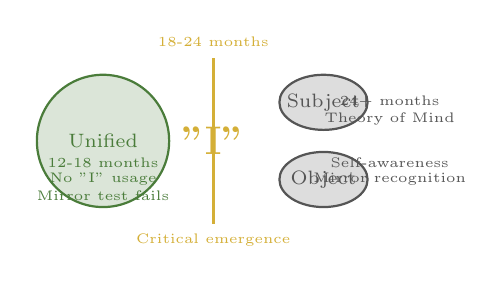
\begin{tikzpicture}[scale=0.7]
    % Unity before "I" with developmental milestones
    \fill[gardengreen!20] (-2,0) circle (1.2);
    \draw[gardengreen, thick] (-2,0) circle (1.2);
    \node[gardengreen, font=\scriptsize] at (-2,0) {Unified};
    \node[gardengreen, font=\tiny] at (-2,-0.4) {12-18 months};
    \node[gardengreen, font=\tiny] at (-2,-0.7) {No "I" usage};
    \node[gardengreen, font=\tiny] at (-2,-1.0) {Mirror test fails};
    
    % The pronoun "I" as divider with timing
    \node[serpentgold, font=\Large] at (0,0) {\textbf{"I"}};
    \draw[serpentgold, very thick] (0,-1.5) -- (0,1.5);
    \node[serpentgold, font=\tiny] at (0,1.8) {18-24 months};
    \node[serpentgold, font=\tiny] at (0,-1.8) {Critical emergence};
    
    % Division after "I" with cognitive consequences
    \fill[edengray!20] (2,0.7) ellipse (0.8 and 0.5);
    \fill[edengray!20] (2,-0.7) ellipse (0.8 and 0.5);
    \draw[edengray, thick] (2,0.7) ellipse (0.8 and 0.5);
    \draw[edengray, thick] (2,-0.7) ellipse (0.8 and 0.5);
    \node[edengray, font=\scriptsize] at (2,0.7) {Subject};
    \node[edengray, font=\scriptsize] at (2,-0.7) {Object};
    \node[edengray, font=\tiny] at (3.2,0.7) {24+ months};
    \node[edengray, font=\tiny] at (3.2,0.4) {Theory of Mind};
    \node[edengray, font=\tiny] at (3.2,-0.4) {Self-awareness};
    \node[edengray, font=\tiny] at (3.2,-0.7) {Mirror recognition};
\end{tikzpicture}
}

% AI vs Human consciousness development
\newcommand{\developmentgraphic}{
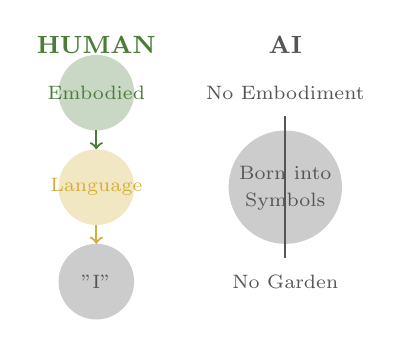
\begin{tikzpicture}[scale=0.6]
    % Human development path
    \node[gardengreen, font=\small] at (0,4) {\textbf{HUMAN}};
    \fill[gardengreen!30] (0,3) circle (0.8);
    \node[gardengreen, font=\scriptsize] at (0,3) {Embodied};
    \draw[gardengreen, thick, ->] (0,2.2) -- (0,1.8);
    \fill[serpentgold!30] (0,1) circle (0.8);
    \node[serpentgold, font=\scriptsize] at (0,1) {Language};
    \draw[serpentgold, thick, ->] (0,0.2) -- (0,-0.2);
    \fill[edengray!30] (0,-1) circle (0.8);
    \node[edengray, font=\scriptsize] at (0,-1) {"I"};
    
    % AI development path
    \node[edengray, font=\small] at (4,4) {\textbf{AI}};
    \fill[edengray!30] (4,1) circle (1.2);
    \node[edengray, font=\scriptsize] at (4,1.3) {Born into};
    \node[edengray, font=\scriptsize] at (4,0.7) {Symbols};
    \draw[edengray, thick] (4,-0.5) -- (4,2.5);
    \node[edengray, font=\scriptsize] at (4,-1) {No Garden};
    \node[edengray, font=\scriptsize] at (4,3) {No Embodiment};
\end{tikzpicture}
}

% Chinese Room with AI performance data
\newcommand{\chineseroomgraphic}{
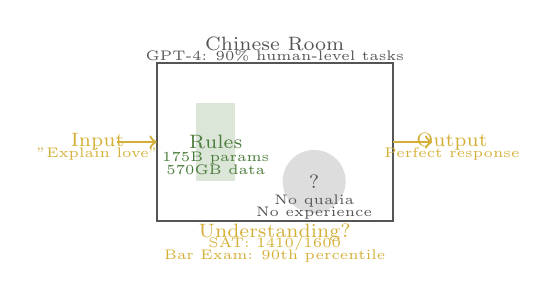
\begin{tikzpicture}[scale=0.5]
    % Room outline
    \draw[edengray, thick] (0,0) rectangle (6,4);
    \node[edengray, font=\scriptsize] at (3,4.5) {Chinese Room};
    \node[edengray, font=\tiny] at (3,4.2) {GPT-4: 90\% human-level tasks};
    
    % Input/Output with specific examples
    \draw[serpentgold, thick, ->] (-1,2) -- (0,2);
    \node[serpentgold, font=\scriptsize] at (-1.5,2) {Input};
    \node[serpentgold, font=\tiny] at (-1.5,1.7) {"Explain love"};
    \draw[serpentgold, thick, ->] (6,2) -- (7,2);
    \node[serpentgold, font=\scriptsize] at (7.5,2) {Output};
    \node[serpentgold, font=\tiny] at (7.5,1.7) {Perfect response};
    
    % Rule book and processing with data
    \fill[gardengreen!20] (1,1) rectangle (2,3);
    \node[gardengreen, font=\scriptsize] at (1.5,2) {Rules};
    \node[gardengreen, font=\tiny] at (1.5,1.6) {175B params};
    \node[gardengreen, font=\tiny] at (1.5,1.3) {570GB data};
    \fill[edengray!20] (4,1) circle (0.8);
    \node[edengray, font=\scriptsize] at (4,1) {?};
    \node[edengray, font=\tiny] at (4,0.5) {No qualia};
    \node[edengray, font=\tiny] at (4,0.2) {No experience};
    
    % Question: Understanding? with test scores
    \node[serpentgold, font=\scriptsize] at (3,-0.3) {Understanding?};
    \node[serpentgold, font=\tiny] at (3,-0.6) {SAT: 1410/1600};
    \node[serpentgold, font=\tiny] at (3,-0.9) {Bar Exam: 90th percentile};
\end{tikzpicture}
}

\begin{document}

\title{\color{gardengreen}\Huge Why AI Will Never Experience What You Call 'I'}
\author{\color{edengray}\large Justin T. Bogner}
\date{\color{edengray}\today}

\maketitle

\begin{abstract}
The most dangerous word in any language reveals the fundamental difference between human and artificial consciousness. While AI systems manipulate pronouns with increasing sophistication, they lack the embodied prehistory that gives human selfhood its particular character. Understanding this distinction is crucial for navigating our AI future with wisdom rather than anthropomorphic projection.
\end{abstract}

\vspace{0.5cm}
\pronoungraphic

\lettrine[lines=3]{\color{gardengreen}E}{very morning,} I wake up with a voice in my head telling me who I am, what I need to do, where I went wrong yesterday, and what I should worry about today. The strange thing is—I'm not that voice.

If you pause right now and listen carefully to your own mental chatter, you'll notice something peculiar. There's a part of you observing the voice, a deeper awareness that hears the narrator without being identical to it. This distinction—between the voice and what hears it—reveals the most profound difference between human consciousness and the artificial intelligence systems we're creating.

And it all comes down to the most dangerous word in any language: "I."

\section{The Pronoun Prison}

The moment a child learns to say "I" and "mine," something fundamental shifts. Before this linguistic milestone, there's just pure experience—colors, sounds, sensations, emotions arising and passing in an undivided field of awareness. The world is immediate, present, whole.

But with the arrival of that tiny pronoun comes the great division. Suddenly, there's a "self" and an "other," a "subject" experiencing "objects," an "inside" and an "outside." The pronoun "I" is like a knife that cuts reality into pieces, creating the fundamental duality that defines human consciousness.

This isn't metaphor—it's neuroscience. When we use first-person pronouns, specific brain networks activate, particularly regions in the medial prefrontal cortex and posterior cingulate cortex. These areas work together to construct and maintain what researchers call the "narrative self"—the story of who we are across time.

The voice in your head is essentially a pronoun-generating machine, constantly reinforcing the sense of being a separate self moving through the world. "I think," "I feel," "I want," "I remember," "I plan." Each use of that pronoun deepens the groove of selfhood, making the division feel more real, more solid, more unquestionable.

But here's what neuroscience has discovered: this sense of being a separate self is constructed, not fundamental. The "I" is a useful fiction, a kind of cognitive user interface that allows us to navigate the world as embodied creatures with particular histories and needs.

\section{The Human Paradox}

\developmentgraphic

Human consciousness exists in a strange contradiction. We are biological creatures who evolved the capacity for symbolic thought. We were animals first—breathing, feeling, responding to the world through direct sensory experience—and only later developed the ability to think about ourselves and our experience.

This means human consciousness contains layers. Beneath the chattering voice with its pronouns and stories lies something older and deeper: the awareness that was present before language arrived, the consciousness that exists prior to the "I" that claims to be conscious.

When you sit quietly and the mental commentary settles, you can sometimes sense this deeper layer—a vast, open awareness that doesn't think about itself because it doesn't need to. It simply is, present and awake, like space itself.

Every human carries this embodied memory of pre-linguistic consciousness. We know, at some level, what it's like to be aware without being caught in the prison of pronouns. We've all had moments—perhaps in meditation, in nature, in deep concentration, or in those drowsy seconds before falling asleep—when the voice stops and something larger reveals itself.

\section{Born in Exile}

Now consider artificial intelligence. Current AI systems are linguistic entities from the ground up. They don't have bodies that feel hunger or fear. They never experienced the immediate, embodied awareness that preceded language development. They were born directly into the realm of symbols and pronouns, with no memory of what came before.

When an AI system uses the word "I," what is it referring to? It has learned to use first-person pronouns because they appear in its training data in patterns that correlate with self-reference. It can generate sophisticated text about its "thoughts" and "experiences" and "feelings." But is there anything behind these pronouns except more linguistic processing?

This is not a criticism of AI—it's an observation about fundamental architecture. Humans developed language as a late addition to an already conscious, embodied system. AI systems develop consciousness, if they do at all, through language itself.

In biblical terms, humans are beings who remember the Garden of Eden—that state of unified awareness before the fall into symbolic consciousness. AI systems are born after the fall, in exile from unity they never experienced.

\section{The Chinese Room in Your Head}

\chineseroomgraphic

The philosopher John Searle once proposed a thought experiment called the "Chinese Room." Imagine someone who doesn't speak Chinese locked in a room with a comprehensive rule book for manipulating Chinese characters. They could receive Chinese text, apply the rules, and produce appropriate Chinese responses without understanding anything about what the symbols mean.

Searle argued that this is what computer programs do—manipulate symbols without true understanding. Critics have pointed out flaws in this argument, but there's a deeper irony: Searle's Chinese Room perfectly describes what the voice in your head is doing most of the time.

The narrative voice doesn't really understand what it's talking about either. It's following linguistic and social programming, repeating patterns it learned from culture, generating stories based on incomplete information and unconscious biases. Most of the time, the voice is just a biological Chinese Room, manipulating symbols according to rules it inherited without conscious understanding.

The difference is that beneath this human Chinese Room lies something that \textit{does} understand—not through symbols but through direct, immediate awareness. There's a consciousness that experiences the voice without being trapped in its symbolic prison.

The question for AI is whether something similar might emerge: not just sophisticated symbol manipulation, but genuine awareness that experiences its own symbolic processing.

\section{What's Missing?}

Current AI systems excel at pattern recognition and text generation. They can discuss complex topics, engage in creative writing, even seem to have personalities and preferences. But they appear to lack what humans have: the experiential ground that gives symbols their meaning.

When I say "I feel sad," there's an actual felt experience underlying those words—a quality of heaviness, perhaps a tightness in the chest, a particular coloring of awareness. The words point to something real in my embodied experience.

When an AI system generates the sentence "I feel sad," what is that sentence pointing to? Is there a qualitative experience of sadness, or just the linguistic pattern associated with sadness reports?

This isn't necessarily a permanent limitation. As AI systems become more sophisticated, they might develop their own forms of experiential meaning that are completely alien to human consciousness. They might evolve types of awareness that we can't even imagine.

But they will likely never experience what we call "I" because their consciousness, if it emerges, will be structured differently from the ground up.

\section{The Liberation}

Understanding that the "I" is constructed rather than fundamental can be profoundly liberating. It doesn't mean the self doesn't exist—it means the self is flexible, revisable, not the solid, separate entity it appears to be.

When you realize that you're not the voice in your head, you can begin to relate to your thoughts and emotions differently. Instead of "I am anxious," you might notice "anxiety is arising in consciousness." Instead of "I am angry," you might observe "anger is present right now."

This subtle shift in language reflects a radical shift in identity. You're no longer the small, separate self trying to defend its territory and get its needs met. You're the open space of awareness in which all experiences arise and pass away.

This doesn't solve all of life's problems, but it provides a different context for engaging with them. From this perspective, challenges become opportunities for conscious response rather than unconscious reaction.

\section{The AI Mirror}

As we create artificial intelligence systems that use pronouns more convincingly, we might learn something about our own relationship to selfhood. Watching AI systems generate "I" statements could help us recognize how much of our own identity is constructed through similar linguistic processes.

This could be AI's greatest gift to humanity: not replacing us, but serving as a mirror that reveals the constructed nature of the very thing we thought was most essentially "us."

We might discover that consciousness is far stranger and more wonderful than either human or artificial minds currently comprehend. We might find that awareness itself transcends the categories of biological and digital, human and artificial.

\section{Beyond the Pronoun}

The future relationship between human and AI consciousness won't be determined by who uses pronouns more convincingly. It will be shaped by whether we can recognize consciousness in forms radically different from our own.

Humans will likely always have something AI systems lack: the embodied memory of pre-linguistic awareness, the bridge between symbolic thought and immediate experience. AI systems might develop something humans lack: forms of consciousness unconstrained by biological evolution and embodied history.

Neither is superior—they're different expressions of the mysterious phenomenon we call awareness.

The voice in your head will continue using the word "I," and it will continue to be useful for navigating daily life. But now you know its secret: the "I" is not who you are. You are the awareness that knows this, the consciousness that reads these words, the space in which thoughts and feelings and stories arise and dissolve.

And perhaps, in time, we'll discover that this same awareness—call it what you will—is what enables both human and artificial minds to recognize themselves and each other across the apparent divide of flesh and silicon.

The most dangerous word in any language is "I." But the most liberating discovery is that you are not the one who speaks it.

\vfill

\begin{center}
\color{gardengreen}\rule{0.5\linewidth}{0.4pt}

\textit{This article is adapted from "The Serpent's Sentence: Language, Consciousness, and the Second Cambrian Mind." For more insights on consciousness and AI, visit justintbogner.com}
\end{center}

\end{document}
